\documentclass[12pt]{tdtp}
\usepackage{tabularx,colortbl}
\usepackage{multirow}
\usepackage{listings}
\lstset{
	language=VHDL,
basicstyle=\tiny\ttfamily}
\definecolor{light-gray}{gray}{0.96}
\definecolor{pageheading-gray}{gray}{0.2}
\definecolor{dark-gray}{gray}{0.45}
\definecolor{dark-green}{rgb}{0.245,0.121,0.0}

\newcommand{\auteur}{Cedric Lemaitre}
\newcommand{\couriel}{c.lemaitre58@gmail.com}
\newcommand{\promo}{M1 ESI}
\newcommand{\annee}{2016-2017}
\newcommand{\matiere}{Composant programmable}

\newcommand{\tdtp}{TP 3}
\renewcommand{\sujet}{VHDL Design}


\begin{document}
\titre
Nous proposons dans ce tp de réaliser des exemples de composants un peu plus évolués.\\

\textit {NB : all examples should be check using \textbf{test-benchs} and simulatuon tools}

%%%%%%%%%%%%
\Exo

Créer un muptiplexeus avec :
\begin{enumerate}
	\item 2 entrées : data(8),add(3)
	\item 1 sortie : s(1)
	\item 1 CLK pour la synchronisation
\end{enumerate}

\textit{NB : un multiplexeur (abréviation : MUX) est un circuit permettant de concentrer sur une même voie de transmission différents types de liaisons (informatique, télécopie, téléphonie, télétex) en sélectionnant une entrée parmi N. Il possèdera donc N entrées, ainsi qu'une entrée de log2 N bits permettant de choisir quelle entrée sera sélectionnée, et une sortie.}
%%%%%%%%%%%%
\newpage
\Exo
Créez un composent VHDL qui permet de réaliser le même comportement que le le décodeur BCD à cathode commune 74HS58\footnote{\url{http://pdf.datasheetcatalog.com/datasheet/motorola/74LS48.pdf}} décrit par la figure \ref{74HS48} . 
L'exemple d'un décodeur BCD est généralement utilisé pour afficher une valeur sur décimale sur un afficheur 7-segments(voir figure : \ref{7seg}).\\
\\

\begin{figure}[h!]
\begin{center}
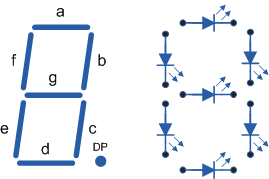
\includegraphics[scale=0.5]{images/7seg.png}
\caption{Exemple d'afficheur 7 segments}
\label{7seg}
\end{center}
\end{figure}


\begin{figure}[h!]
\begin{center}
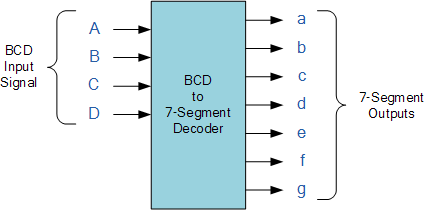
\includegraphics[scale=0.5]{images/74LS48.png}
\caption{Décodeur BCD}
\label{74HS48}
\end{center}
\end{figure}

\textit{NB : Les afficheurs 7 segments sont un type d'afficheur très présent sur les calculatrices et les montres à affichage numérique : les caractères (des chiffres, bien que quelques lettres soient utilisées pour l'affichage hexadécimal) s'écrivent en allumant ou en éteignant des segments, au nombre de sept. Quand les 7 segments sont allumés, on obtient le chiffre 8.}

%%%%%%%%%%%%
\end{document}
